\documentclass{article}
\usepackage{tikz}
\usetikzlibrary{tqft}

\begin{document}

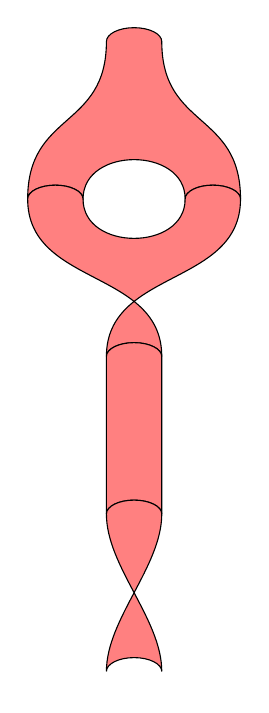
\begin{tikzpicture}[tqft/cobordism/.style={draw,fill=red!50}]

\pic[tqft/pair of pants,name=a];
\pic[tqft/reverse pair of pants,twisted,anchor={(incoming boundary 1)},at={(a-outgoing boundary 1)},name=b];
\pic[tqft/cylinder,name=c,anchor={(incoming boundary 1)},at={(b-outgoing boundary 1)}];
\pic[tqft/cylinder,twisted,name=d,anchor={(incoming boundary 1)},at={(c-outgoing boundary 1)}];

\end{tikzpicture}

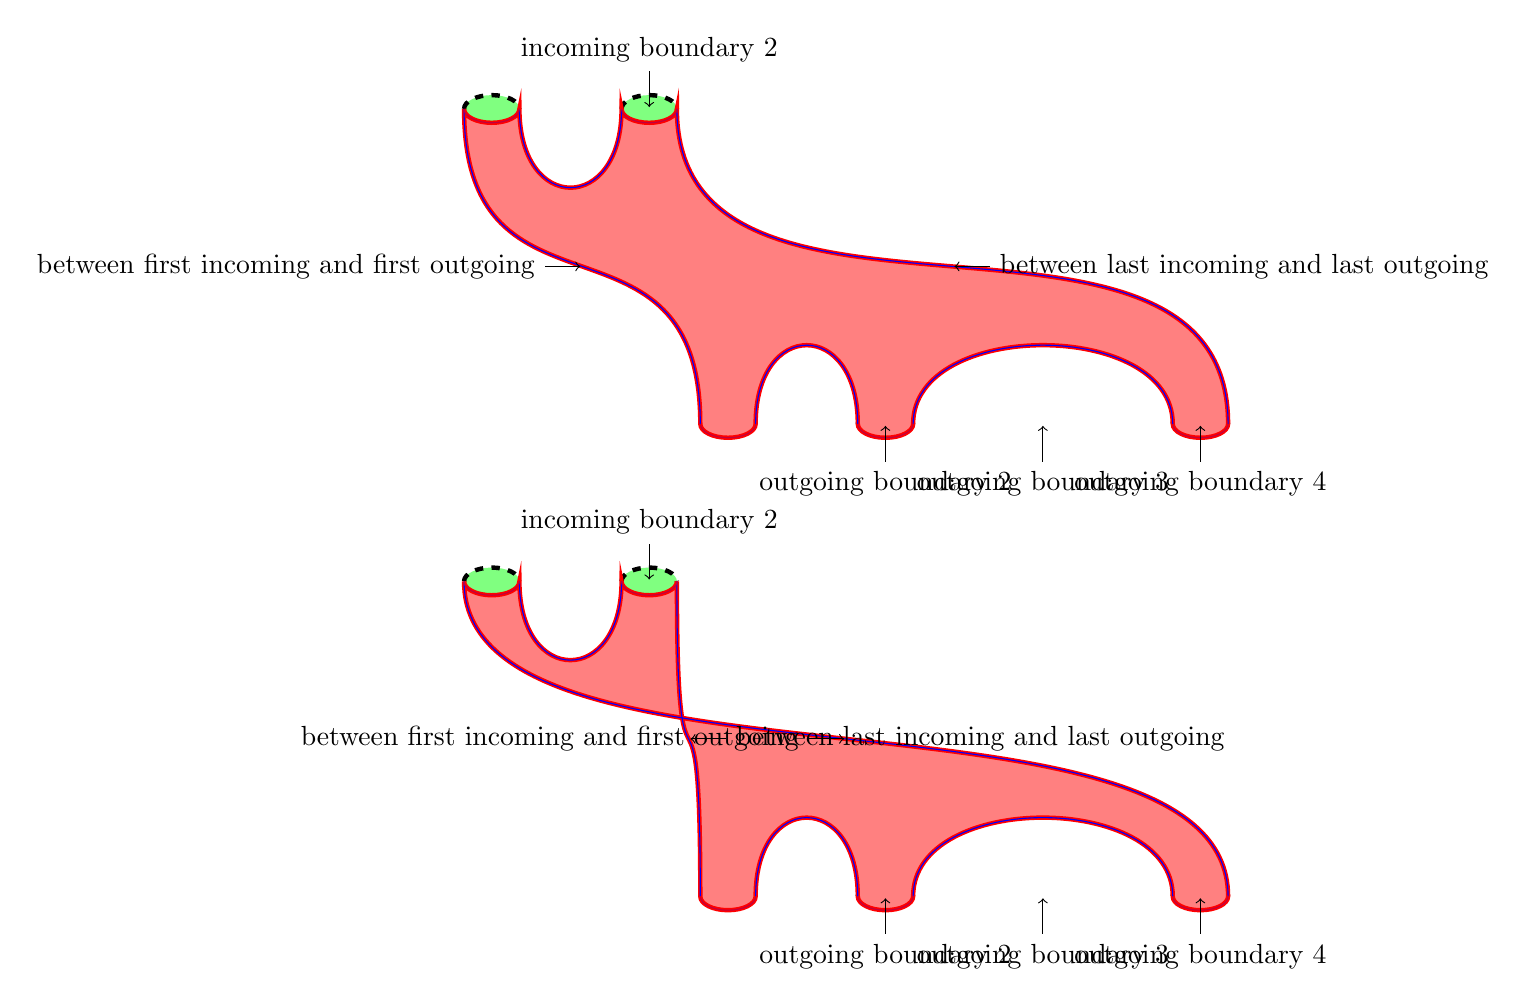
\begin{tikzpicture}[
  tqft,
  every outgoing boundary component/.style={fill=blue!50},
  outgoing boundary component 3/.style={fill=none,draw=red},
  every incoming boundary component/.style={fill=green!50},
  every lower boundary component/.style={draw,ultra thick, dashed},
  every upper boundary component/.style={draw,purple},
  cobordism/.style={fill=red!50,draw=red, ultra thick},
  cobordism edge/.style={draw,blue},
  view from=incoming,
  cobordism height=4cm,
  offset=1.5,
  incoming boundary components=2,
  outgoing boundary components=4,
  skip outgoing boundary components=3
]
\pic[
  name=a,
  tqft,
];
\pic[
  name=b,
  at={(0,-6)},
  tqft,
  twisted,
];

\begin{scope}[every pin edge/.style={<-}]
\foreach \cobordism in {a,b}
{
\foreach \anchor/\ang in {
%  hole 1/-90,
%  hole 2/90,
%  hole 3/-90,
  incoming boundary 2/90,
  outgoing boundary 2/-90,
  outgoing boundary 3/-90,
  outgoing boundary 4/-90,
  between last incoming and last outgoing/0,
  between first incoming and first outgoing/180%,
%  between incoming 1 and 3/90,
%  between outgoing 1 and 4/-90,
%  between outgoing 4 and 6/-90
} {
  \node[pin=\ang:\anchor,at=(\cobordism-\anchor),inner sep=0pt] {};
  }
  }
\end{scope}
\end{tikzpicture}
\end{document}
